\documentclass[12pt]{article}
\usepackage[top=1in, bottom=1in, left=1in, right=1in]{geometry}

\usepackage{setspace}
\onehalfspacing

\usepackage{amssymb}
%% The amsthm package provides extended theorem environments
\usepackage{amsthm}
\usepackage{epsfig}
\usepackage{times}
\renewcommand{\ttdefault}{cmtt}
\usepackage{amsmath}
\usepackage{graphicx} % for graphics files

% Draw figures yourself
\usepackage{tikz} 

% writing elements
\usepackage{mhchem}

\usepackage{paralist}

% The float package HAS to load before hyperref
\usepackage{float} % for psuedocode formatting
\usepackage{xspace}

% from Denovo Methods Manual
\usepackage{mathrsfs}
\usepackage[mathcal]{euscript}
\usepackage{color}
\usepackage{array}

\usepackage[pdftex]{hyperref}
\usepackage[parfill]{parskip}

% math syntax
\newcommand{\nth}{n\ensuremath{^{\text{th}}} }
\newcommand{\ve}[1]{\ensuremath{\mathbf{#1}}}
\newcommand{\Macro}{\ensuremath{\Sigma}}
\newcommand{\rvec}{\ensuremath{\vec{r}}}
\newcommand{\omvec}{\ensuremath{\hat{\Omega}}}
\newcommand{\vOmega}{\ensuremath{\hat{\Omega}}}

\newlength\Colsep
\setlength\Colsep{10pt}
%---------------------------------------------------------------------------
%---------------------------------------------------------------------------
\begin{document}
\begin{center}
{\bf NE 155/255, Fall 2019\\
Transport Equation Conditions and Simplifications\\
September 18, 2019}
\end{center}

\setlength{\unitlength}{1in}
\begin{picture}(6,.1) 
\put(0,0) {\line(1,0){6.25}}         
\end{picture}

\subsection*{Additional Conditions}
\begin{itemize}
\item Finiteness condition: $0 \leq \psi(\vec{r}, E, \vOmega, t) \leq \infty$
\item Interface condition: $\psi_1(\vec{r}, E, \vOmega, t) = 
      \psi_2(\vec{r}, E, \vOmega, t) \qquad \forall \vec{r} \in S_i$, all 
      energies, and all $\vOmega$
\item Source condition: $Q(\vec{r_0}, E, \vOmega, t) =
      Q_0(E, \vOmega, t)\delta(\vec{r} - \vec{r_0})$
\end{itemize}

\begin{figure}[h!]
    \begin{center}
    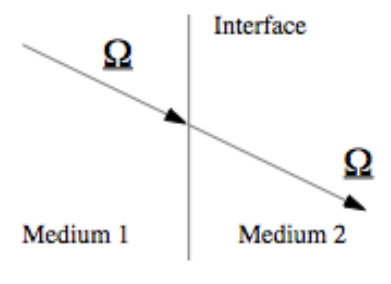
\includegraphics[keepaspectratio, width = 1.5 in]{interface}
     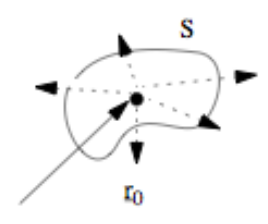
\includegraphics[keepaspectratio, width = 1.5 in]{source}
    \end{center}
\end{figure}

%----------------------------------------------
\section*{Simplified Forms}

\subsection*{Time Independence}

We assume that losses and sources are balanced, and thus there is no rate of change with time:

\[\frac{\partial \psi}{\partial t} = 0\]

We can then remove the time dependence from all terms in our equation. As 
noted, for reactors we often 

\begin{compactitem}
\item solve a steady-state form of the equation,
\item perform depletion calculations that characterize material evolution
      (using the Batemann equations, which we're skipping for now)
\item solve a new steady-state calculation with updated material 
      specifications.
\end{compactitem}

\subsection*{One Speed}

Assume all particles are at the same speed, $\vec{v} = v_0 \cdot \vOmega$. Then

\begin{align*}
n(\vec{r}, v, \vOmega, t) &= n(\vec{r}, \vOmega, t) \delta(v - v_0) \\
\Sigma_s(E' \rightarrow E, \vOmega' \rightarrow \vOmega) &=
\Sigma_s(E, \vOmega' \rightarrow \vOmega)\delta(E' - E)
\end{align*}

Now we can remove E integration and E dependence:

\begin{align*}
\frac{1}{v}\frac{\partial \psi(\vec{r}, \vOmega, t)}{\partial t} &+ 
\vOmega \cdot \nabla \psi(\vec{r}, \vOmega, t) +
\Sigma_t \psi(\vec{r}, \vOmega, t) = \nonumber\\
%
& \int_{4\pi} d\vOmega' \Sigma_s(\vOmega' \rightarrow \vOmega)
\psi(\vec{r}, \vOmega', t)  
+ \frac{\nu \Sigma_f}{4\pi} \int_{4\pi} d\vOmega' \psi(\vec{r},  \vOmega', t) 
+ S(\vec{r}, \vOmega, t) 
%Q(\vec{r}, \vOmega, t)
\end{align*}
%
%Where:
%\begin{align}
%Q(\vec{r}, \vOmega, t) &= \frac{1}{4\pi} \nu \Sigma_f \int_{4\pi} d\vOmega' \psi(\vec{r},  \vOmega, t) + S(\vec{r}, \vOmega, t) \\
%&= \frac{1}{4\pi} \bigl( \nu \Sigma_f \phi(\vec{r}, t) + s(\vec{r}, t) \bigr)
%\end{align}

\subsection*{Isotropic Source}

It is often the case that an external source is (or we can approximate it as)
isotropic:

\[ S(\vec{r}, E, \vOmega, t) = \frac{1}{4 \pi}  S(\vec{r}, E, t) \]

%---------------------------------------------
\subsection*{One Dimensional and Rotational (Azimuthal) Symmetry}

We also often simplify by only worrying about fewer dimensions. Here we'll 
look at just one: we'll get rid of $x$ and $y$. 

We first assume that \textbf{things only vary in the $z$ dimension}, so
$\vec{r} \rightarrow z$, e.g.
$\psi(\vec{r}, E, \vOmega, t) \rightarrow \psi(z, E, \vOmega, t)$

We next assume (which is often true) that our systems is \textbf{azimuthally
symmetric}, which means that the scattering is symmetric about the azimuthal
direction ($\varphi$). Therefore, scattering only depends on the angle of the
scattering cosine, $\mu_0 =\vOmega' \cdot \vOmega$, the angle between where it
was heading and where it is heading. We can use this assumption to simplify
two things. 

\noindent\begin{minipage}{\textwidth}
\begin{minipage}[c][6cm][c]{\dimexpr0.5\textwidth-0.5\Colsep\relax}
    \begin{center}
    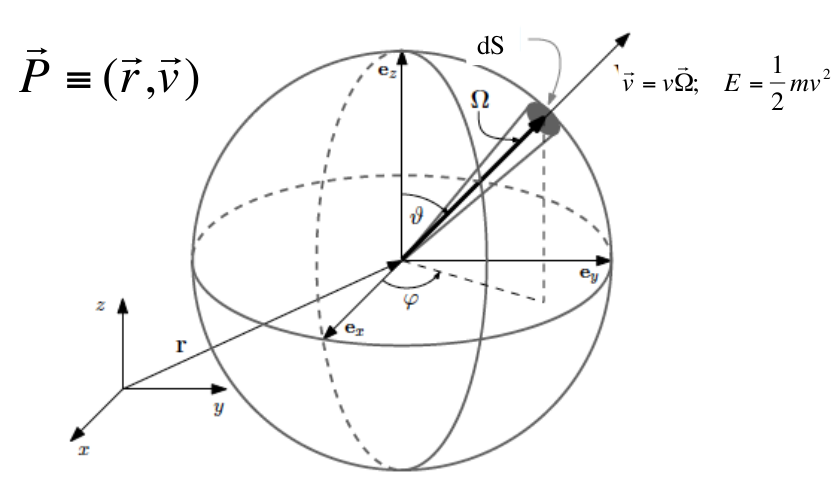
\includegraphics[keepaspectratio, width = 3 in]{phase-space}
    \end{center}
\end{minipage}\hfill
\begin{minipage}[c][6cm][c]{\dimexpr0.5\textwidth-0.5\Colsep\relax}
\begin{gather*}
d\vOmega = \sin(\theta) d\theta d\varphi = d\mu d\varphi \\
\mu = \cos(\theta), \text{ so } d\mu = \sin(\theta)d\theta \\
\Omega_z = \cos(\theta) = \mu
\end{gather*}
\end{minipage}%
\end{minipage}


Recall our new definition $\mu_0 = \vOmega' \cdot \vOmega$.

\begin{gather*}
\int_{4 \pi} d\vOmega =
\int_0^{2\pi} d\varphi \int_{0}^{\pi} \sin(\theta) d\theta = 
\int_0^{2\pi} d\varphi \int_{-1}^1 d\mu = 4\pi \\
\psi(z,\vOmega,E,t) d\vOmega = \psi(z,\varphi, \mu,E,t) d\varphi  d\mu =
\psi(z, \mu,E,t) d\varphi  d\mu 
\end{gather*}

With azimuthal symmetry, we can rewrite the scattering cross section since it
is no longer a function of $\varphi$.

\[\Sigma_s(z, E' \rightarrow E, \vOmega' \rightarrow \vOmega) \rightarrow
\Sigma_s(z, E' \rightarrow E, \vOmega' \cdot \vOmega) = \Sigma_s(z, E' \rightarrow E, \mu_0) \:.\]

Further, we can execute the angular integration over $\varphi$ since nothing
depends on it anymore:

\[\int_{4 \pi} d\vOmega\: \psi(z, \vOmega, E, t) =
\int_0^{2\pi} d\varphi \int_{-1}^1 d\mu \:\psi(z, \vOmega, E, t) =
2 \pi \int_{-1}^1 d\mu \:\psi(z, \mu, E, t)\:.\]

The next simplification is in the streaming term:

\[\vOmega \cdot \nabla \psi(\vec{r}, \vOmega, E, t) \rightarrow
\Omega_z \frac{\partial \psi(z, \mu, E, t)}{\partial z} =
\mu \frac{\partial \psi(z, \mu, E, t)}{\partial z} \]

We can combine all of this into a 1-D equation, using
$\mu_0 = \vOmega' \cdot \vOmega$:

\begin{align*}
\frac{1}{v}\frac{\partial \psi}{\partial t}(z,E,\omvec,t) &+
\Omega_z \frac{\partial \psi(z, \vOmega, E, t)}{\partial z} +
\Sigma_t(z)\psi(z, \vOmega, E, t)  \\
&= \frac{\chi(E)}{4 \pi} \int_0^{\infty} dE'\int_{4 \pi} d\vOmega'\: 
\nu(E')\Sigma_f(z,E',t)\psi(z, \vOmega', E', t)  \\
&+ \int_0^{\infty} dE' \int_{4 \pi} d\vOmega'\:
\Sigma_s(z, E' \rightarrow E, \mu_0)\psi(z, \vOmega', E', t) + S(z, E, \vOmega, t)\:,
\end{align*}

which we can then integrate over the $\varphi$ component of angle:

\begin{align*}
\frac{1}{v}\frac{\partial \psi}{\partial t}(z,E,\mu,t) &+
\mu \frac{\partial \psi(z, \mu, E, t)}{\partial z} +
\Sigma_t(z)\psi(z, \mu, E, t) \\
&= 2\pi\frac{\chi(E)}{4 \pi} \int_0^{\infty} dE' \:
\nu(E')\Sigma_f(z,E') \int_{-1}^1 d\mu'\: \psi(z, \mu', E', t) \\
&+ 2\pi\int_0^{\infty} dE' \int_{-1}^1 d\mu'\:
\Sigma_s(z, E' \rightarrow E, \mu_0)\psi(z, \mu', E', t)  + S(z, E, \mu, t)
\end{align*}

Note that the fission term becomes

\[\frac{\chi(E)}{2} \int_0^{\infty} dE'\:
\nu(E')\Sigma_f(z,E')\underbrace{\phi(z, E', t)}_{\text{scalar flux}}\:. \]

\subsection*{Combination}

If we combine one-speed, time-independent, isotropic source, one-dimensional,
and azimuthally-symmetric, we get

\begin{align*}
\mu \frac{\partial \psi(z, \mu)}{\partial z} &+
\Sigma_t(z)\psi(z, \mu) = \\
&\frac{\nu\Sigma_f(z) }{2}\phi(z) + 2\pi\int_{-1}^1 d\mu'\:
\Sigma_s(z, \mu_0)\psi(z, \mu')  + \frac{S(z)}{2} \:.
\end{align*}

\end{document}